

\section{Background}
\label{sec:background}

We first present an example of commit change motivating our deep learning framework. We then briefly introduce a background knowledge about Convolutional Neural Network (CNN) used to extract features in the commit change. 

\subsection{Code changes}\label{sec:examle}
\begin{figure}[t!]
\center
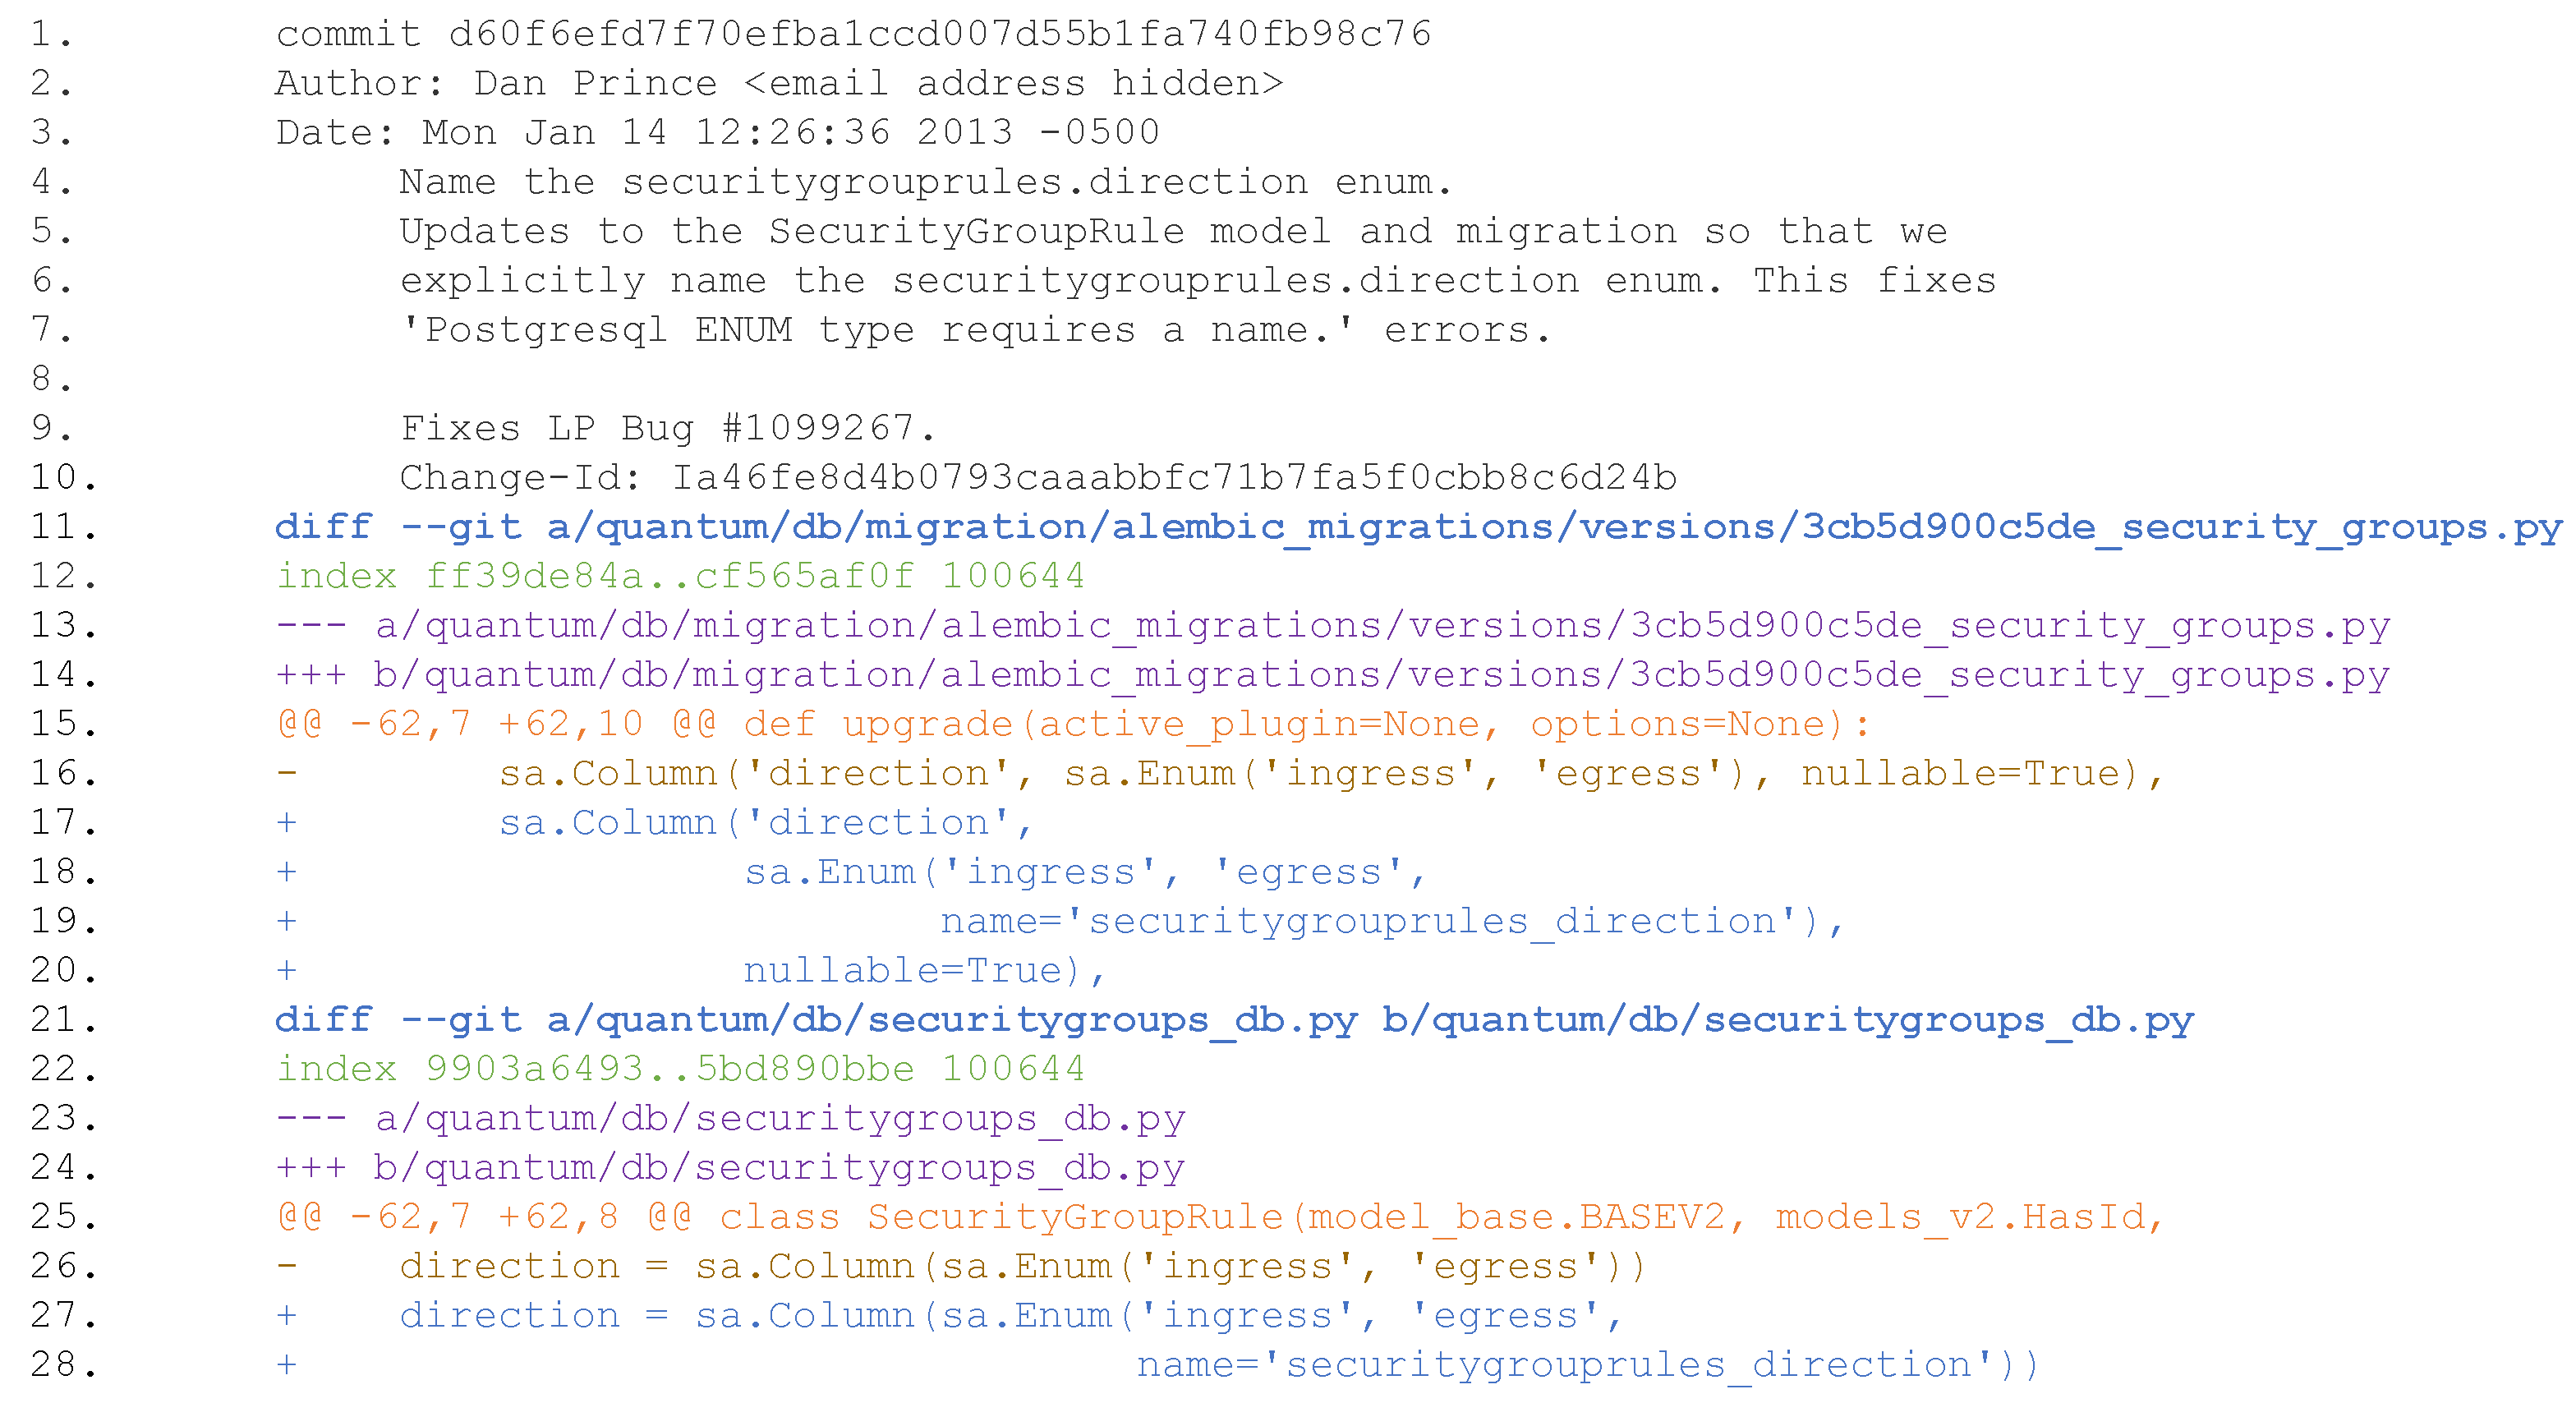
\includegraphics[scale=0.2]{figs/example.pdf}
\caption{An example of a buggy commit change.}
\label{fig:example}
\end{figure} 
Figure~\ref{fig:example} shows a sample of a buggy commit. The buggy commit contains many pieces of information, i.e., a commit id (line 1), a author name (line 2), a commit date (line 3), a commit message (line 4-10) and a set of code changes (i.e., 11-28). The commit message plays an important role when you commit your change since it is the first thing people will see about the change. A good commit message can help maintainers to speed up the reviewing process and write a good release note. A set of code changes includes changes of multiple files and each file includes a number of deleted and added lines representing the change. In the Figure~\ref{fig:example}, line 16 (starting with \texttt{-}) and line 17-20 (starting with \texttt{+}) indicates the deleted and added lines of a change file (namely \texttt{3cb5d900c5de\_security\_groups.py}), respectively. 

Previous works mainly depend on a set of manually features extracted from code changes~\cite{Yang:2015:DLJ, mcintosh2018fix}, however, the manual code features might overlook features which find helpful to identify a buggy commit. Moreover, the commit message in the commit is also ignored. Thus, a powerful feature representation of commit message and code changes is needed to detect buggy commits. 

Inspired by a deep learning Convolutional Neural Network (CNN)~\cite{lecun2015deep}, our deep learning \emph{Just-In-Time} (JIT) defect prediction model (DeepJIT) aims to automatically extract features of the commit message and the code changes of a given commit, respectively. These features are then combined to evaluate whether the given commit is buggy. 
% The key challenge here is to capture the semantic and syntactical structure of the code changes in the given commit. 
Different from the commit message, the code changes include a number of deleted and added lines across multiple files (see Figure~\ref{fig:example}). To solve this problem, we first learn the semantic features of each added or deleted line for each changed file using CNN framework, the semantic features of the added and deleted lines are then incorporated to build a new representation 
% preserving the syntactical structure 
of the change file. We again use CNN to extract features from the new representation of the change file. These features of all the change files are used to construct the features of the code changes in the given commit. Section~\ref{sec:approach} briefly describes DeepJIT. 

\subsection{Convolutional Neural Network}
\label{sec:background_cnn}

\begin{figure*}[t!]
	\center
	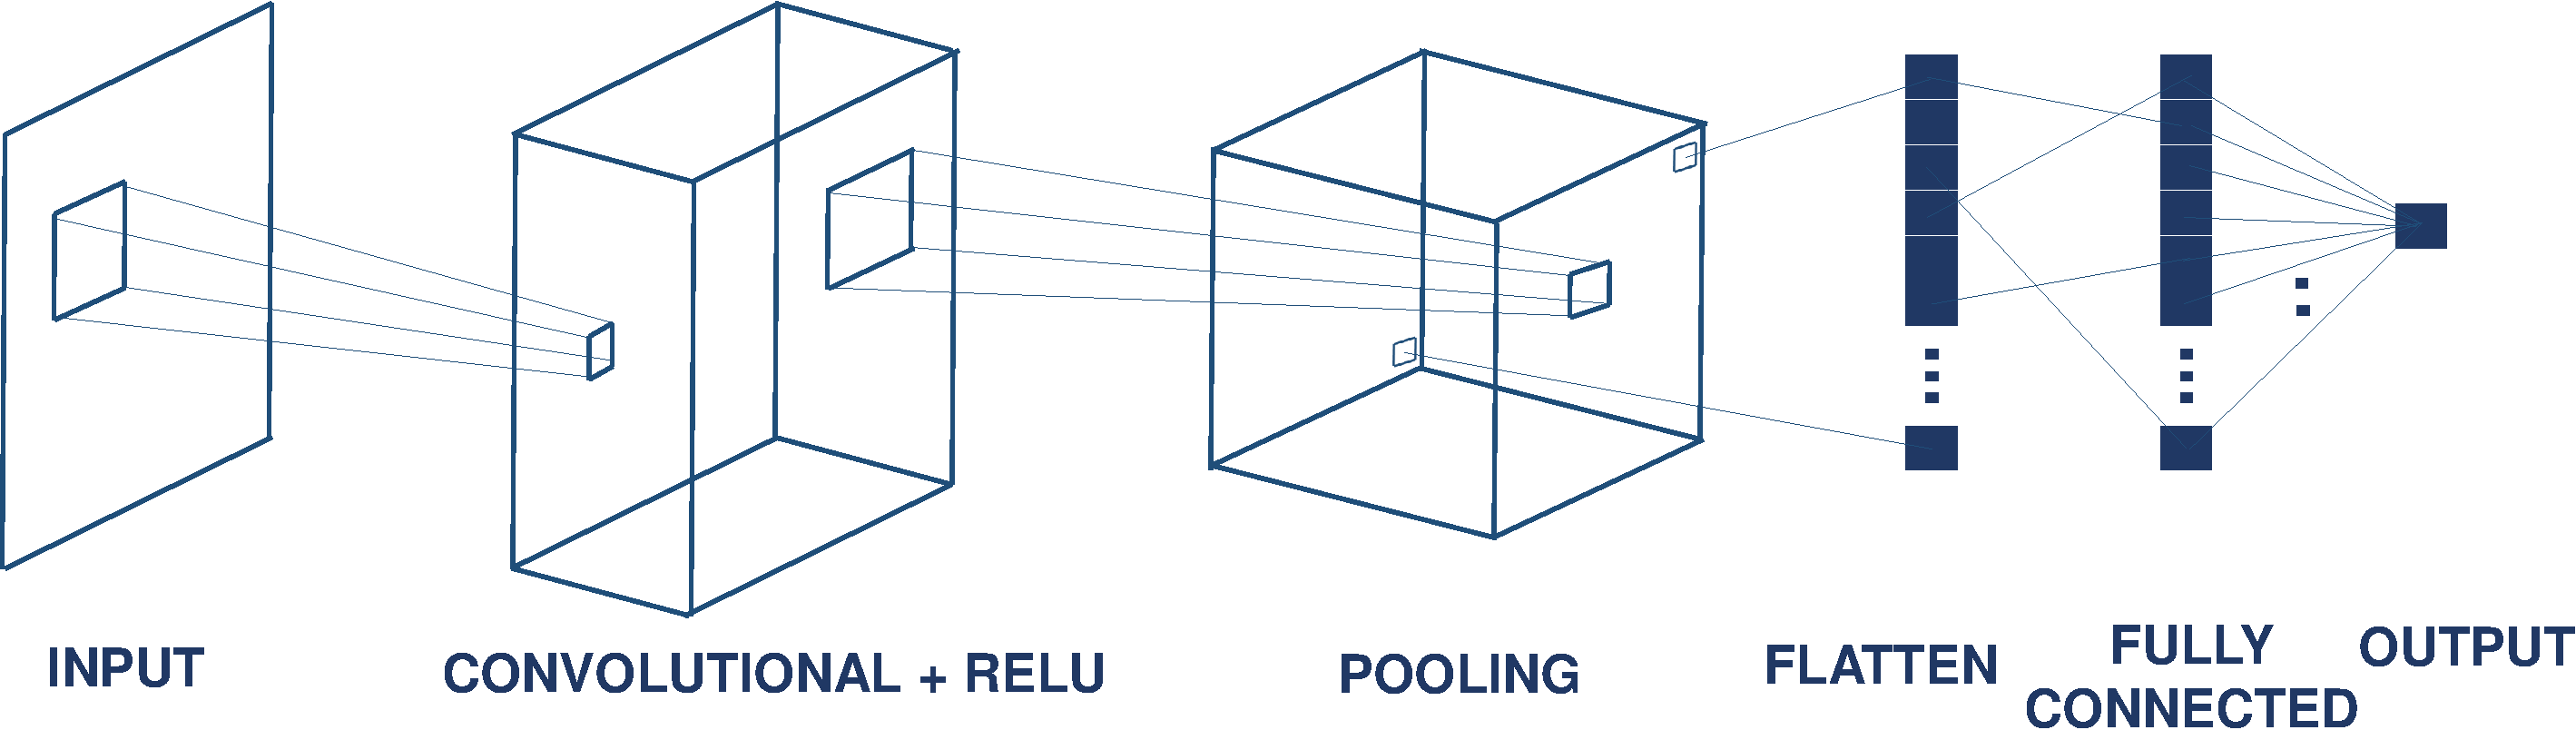
\includegraphics[scale=0.3]{figs/cnn.pdf}
	\caption{A simple convolutional neural network architecture.}
	\label{fig:cnn}
\end{figure*}

\begin{figure*}[t!]
	\center
	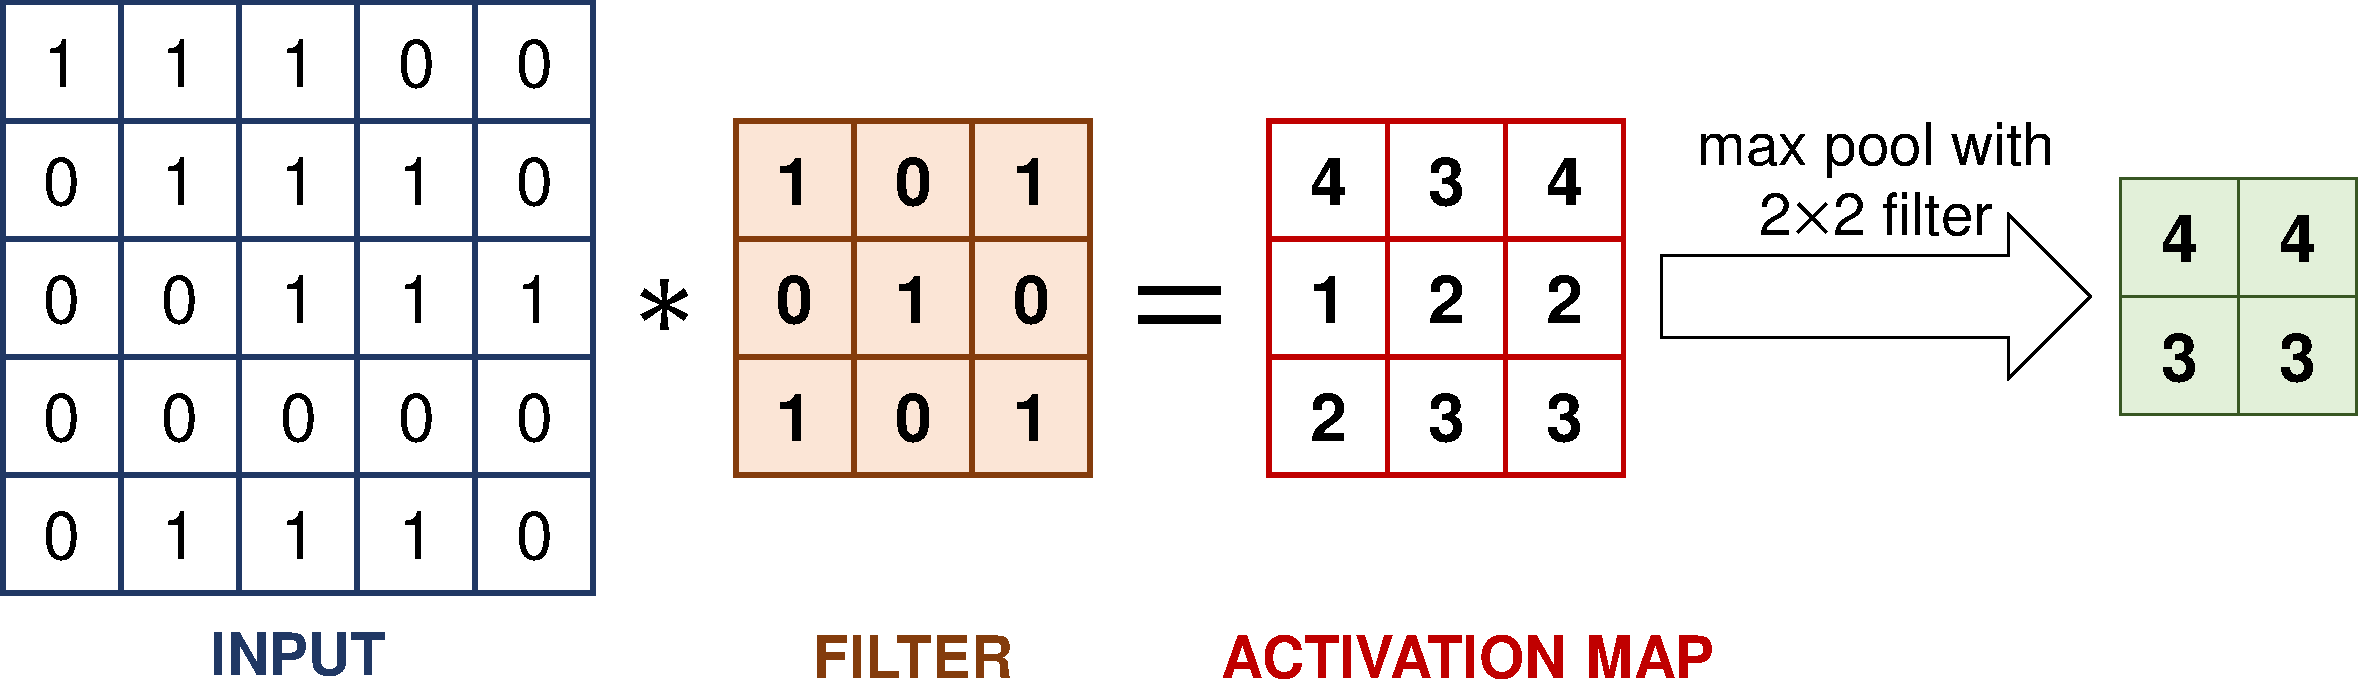
\includegraphics[scale=0.3]{figs/filter_pooling.pdf}
	\caption{An example of a convolutional layer and pooling layer in CNN.}
	\label{fig:filter}
\end{figure*}

One of the most powerful forms of deep learning neural networks is the Convolutional Neural Network (CNN)~\cite{lecun2015deep}. CNNs are widely used to solve image pattern recognition problems and have been achieved significant results~\cite{karpathy2014large, lawrence1997face, krizhevsky2012imagenet}. Like traditional deep learning networks, CNNs receive an input and perform a product operation followed by a nonlinear function. The last layer is the output layer containing objective functions~\cite{zhao2017loss} associated with the labels of the input.

Figure~\ref{fig:cnn} illustrates a simple CNN for classification task. The simple CNN includes an input layer, a convolutional layer, followed by the rectified linear unit (RELU) which is a nonlinear activation function, a pooling layer, a fully-connected layer, and an output layer. We briefly explain these layers in the following paragraphs. 

The input layer takes an input as 2-dimensional array or 3-dimensional array and passes it through a of convolution layers.

The convolutional layer plays a vital role in CNN and it takes advantage of the use of learnable filters. These filters are small in spatial dimensionality, but they are applied along the entirety of the depth of the input data. For example, given an input data $\textbf{I} \in \mathbb{R}^{\text{H} \times \text{W} \times \text{D}}$ and a filter $\textbf{K} \in \mathbb{R}^{\text{h} \times \text{w} \times \text{D}}$, we produce a new activation map $\textbf{A} \in \mathbb{R}^{(\text{H} - \text{h}) \times (\text{W} - \text{w}) \times 1}$. The RELU is then applied to each value of the activation map as follows:
\begin{equation}
\label{eq:relu}
f(x) = max(0, x)   
\end{equation}

The pooling layer, which is an important component of CNN, aims to reduce the dimensionality of the activation map, the number of parameters, and the computational helping to control overfitting problem~\cite{tolias2015particular}. The pooling layer spreads along the activation map and scales its dimensionality. There are three different types of pooling layers:
\begin{itemize}
	\item Max pooling takes the largest element from each region of the activation map.
	\item Average pooling constructs the average value from each region of the activation map.
	\item Sum pooling sums all the elements from each region of the activation map. 
\end{itemize}
In practice, max pooling often achieves a better performance compared to the other two pooling techniques~\cite{zeiler2013stochastic}. Figure~\ref{fig:filter} presents a visual representation of a convolutional layer and pooling layer in CNN. Given an input 5$\times$5 and a filter 3$\times$3, we output a new activation map 3$\times$3. A max pooling layer with a filter 2$\times$2 is then applied to produce a new output. 

The output of pooling layer is flatten and directly passed to a fully connected layer (or a hidden layer). The fully connected layer is passed to an output layer to calculate an objective function (or a loss function)~\cite{zhao2017loss}. The objective function normally is optimized using a stochastic gradient descent (SGD)~\cite{bottou2010large}. This is an analogous way with traditional neural networks~\cite{huang1988neural}.



